\documentclass[12pt]{mitthesis}
\usepackage{lgrind, amsmath, amssymb, longtable, booktabs, subfig,
  color, braket}
\usepackage[pdftex]{graphicx}
\pagestyle{plain}

\newcommand{\TODO} [1]{\textcolor{magenta}{\textbf{TODO:} #1}}
\newcommand{\POINT}[1]{\textcolor{magenta}{\emph{#1}}}

\newcommand{\rcm}{cm$^{-1}$}

\newcommand{\sing}{$S_1\,3\nu_3'$ }
\newcommand{\trip}{$T_3$ }

\newcommand{\strans} {$S_1\,3\nu_3'-S_0(K_0^1)$ }
\newcommand{\atrans} {$S_1\,3\nu_3'-S_0(K_0^0)$ }
\newcommand{\ptrans} {$S_1(3\nu_4'+\nu_6')-S_0(K_0^1)$ }
\newcommand{\fftrans}{$S_1\,4\nu_4'-S_0(K_0^0)$ }
\newcommand{\fstrans}{$S_1\,4\nu_6'-S_0(K_0^0)$ }

\setlongtables
\begin{document}
\tableofcontents
\clearpage

\subsubsection*{NOTES}
\clearpage

\chapter{Evidence for a singlet$\sim$triplet dynamical ``double
  doorway'' in acetylene $\tilde{A} ^1A_u-\tilde{X}^1\Sigma^+_g$
  $V^3_0K^1_0$}

\section{Introduction}
The $\tilde{A} ^1A_u-\tilde{X}^1\Sigma^+_g$ $V^3_0K^1_0$ transition of
acetylene has been heavily studied, in part because it plays host to
several interesting energy resonances.  Firstly, a singlet vibrational
level involving 4 quanta of the Fermi-resonant bending modes $\nu_4$
and $\nu_6$ is near degenerate with $3\nu_3$ at $J=0$.  This singlet
perturber quickly detunes due to a relatively large difference in
rotational constant.  However, due to strong anharmonic and Coriolis
interactions between modes 4 and 6, the singlet level has never been
assigned.  A series of recent ultra-sensitive LIF studies have
resulted in the conclusive assignment of this level as \TODO{Get
  assignment.}

Secondly, a vibrational level of the $T_3$ electronic state crosses
the $S_1$ $3\nu_3$ level near $J=3$.  The interaction between this

\TODO{Include citations: Ryan + Adya (2004), Drabbels (1994), Abramson
  (80's), other triplet SEELEM (90's, 00's), Dupre papers (90's)}

\POINT{Review the data from Mattijs and make the trends in (S1, T3)
  vs. (T1, T2) intensity more apparent.}  Recently, DeGroot \emph{et
  al.} have observed in photoelectron kinetic energy experiments that
the coupling between $S_1$ $3\nu_3$ and the manifold of $T_{1,2}$
states \emph{increases} with rotational quantum number.

\begin{figure}
  %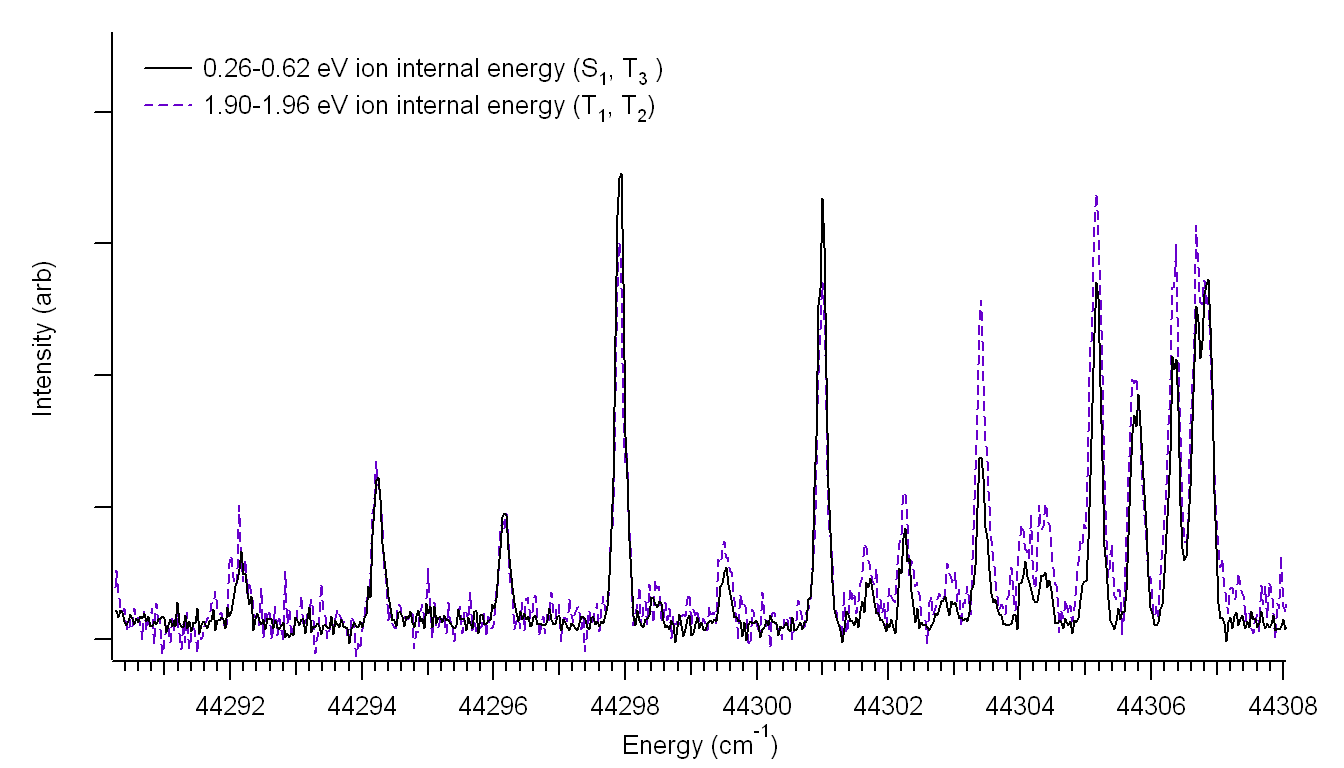
\includegraphics[scale=0.8]{mattijs-traces-2n3.png}
  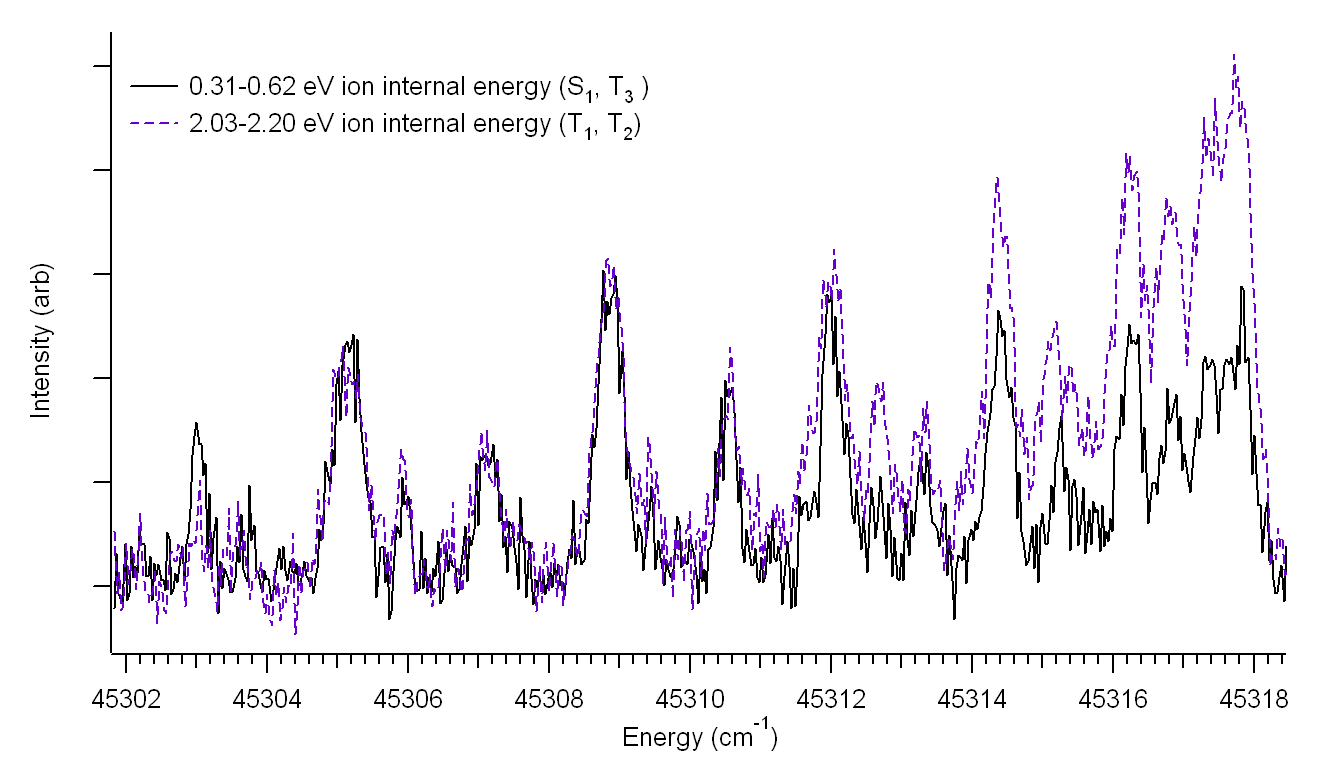
\includegraphics[scale=0.8]{mattijs-traces-3n3.png}
  \caption{Energy-resolved photoelectron intensity from acetylene
    $S_1$ $V^3_0K^1_0$.  \TODO{Get permission to use this data.}}
  \label{fig:mattijs-traces}
\end{figure}

% \POINT{Mention that Mattijs used a 1T magnetic field during his
%   experiments. Derive the energy of the local doorway under these
%   conditions using a $g$ value of 2.}  

A magnetic field of approximately 1 T was used in the energy-resolved
photoelectron experiments.  This has the effect of splitting the
triplet level into three components according to the possible values
of the laboratory-fixed projection of spin, $M_S=0,\pm 1$.  The change
in energy with magnetic field is given by the linear approximation of
the Zeeman effect:
\begin{equation}
  \Delta E = M_S \, g \, \mu_B \, \Delta B,
\end{equation}
where $g$ is the Land\'{e} $g$ factor for the triplet level, and
$\mu_B$=0.4669 cm$^{-1}$/T is the Bohr magneton.  For a triplet level
in the limit of Hund's case ($b$), the $g$ factor is expected to be
close to the ``free electron'' value of 2.0015.  Under the
experimental conditions of DeGroot \emph{et al.}, the magnetic
field-induced splitting in the local $T_3$ perturber is about 1
cm$^{-1}$.

\POINT{}

\POINT{Report the spectroscopic parameters of the local doorway to the
  best of our understanding.}  The matrix element between $S_1$
$3\nu_3$ and the local triplet perturber is approximately $0.1$ \rcm.
We have shown conclusively in the last chapter, by applying a compund
spectral deconvolution technique to high-resolution LIF spectra, that
the local $T_3$ doorway level crosses the $S_1$ $3\nu_3$ $e$-symmetry
levels at $J=3$ and tunes \emph{away} in energy as $J$ increases.  The
rotational constant and...

\POINT{Discuss the assignment of the local $T_3$ pertuber as the $F_2$
  component of a $K_T=1$ level.  An $F_1$ or $F_3$ component with a
  reasonable $B$-value would only be near-resonant with the singlet
  level for a single value of $J$.}

\POINT{Give the resulting dependence of spin-orbit matrix element on
  $J$.}  Stevens and Brand have derived vibronic spin-orbit matrix
elements for polyatomic molecules.  For the $F_2$ component of a local
doorway with $K_T=1$, the spin-orbit matrix element is
\begin{equation}
  \braket{\psi_{S_1}J_S1|H^{SO}|\psi_{T_3}J_S1} = 
  \frac{1}{\sqrt{J_S(J_S+1)}}\braket{\psi_{S_1}|\psi_{T_3}}\braket{H^{SO}(R_z)},
\end{equation}
that is, the spin-orbit matrix element decreases weakly with rotation.
If the local doorway instead has $K_T=0$, the rotational dependence of
the spin-orbit coupling disappears completely: 
\begin{equation}
  \braket{\psi_{S_1}J_S1|H^{SO}|\psi_{T_3}J_S0} =
  \frac{1}{2}\braket{\psi_{S_1}|\psi_{T_3}}
  (\braket{H^{SO}(R_x)} - \braket{H^{SO}(R_y)}).
\end{equation}
Under either circumstance, the spin-orbit interaction is not expected
to increase with rotation.

Therefore, if the local $T_3$ doorway level were the sole mediator for
intersystem crossing between $S_1$ $3\nu_3$ and the manifold of
$T_{1,2}$ levels, one would expect the $S_1 \sim T_{1,2}$ coupling to
decrease with the $S_1 \sim T_3$ energy difference.  The authors
address this issue by proposing that an unobserved, energetically
distant $T_3$ level interacts more strongly with the $S_1$ $3\nu_3$
level.  Interference between the local and distant doorway levels
could cause the $S_1 \sim T_{1,2}$ coupling to decrease in the
vicinity of the local $S_1 \sim T_3$ crossing.



\POINT{Discuss Figure~\ref{fig:mattijs-traces}: Early and late photoelectron
signals from $2\nu'_3$ and $3\nu'_3$.}

\begin{figure}
  \centering
  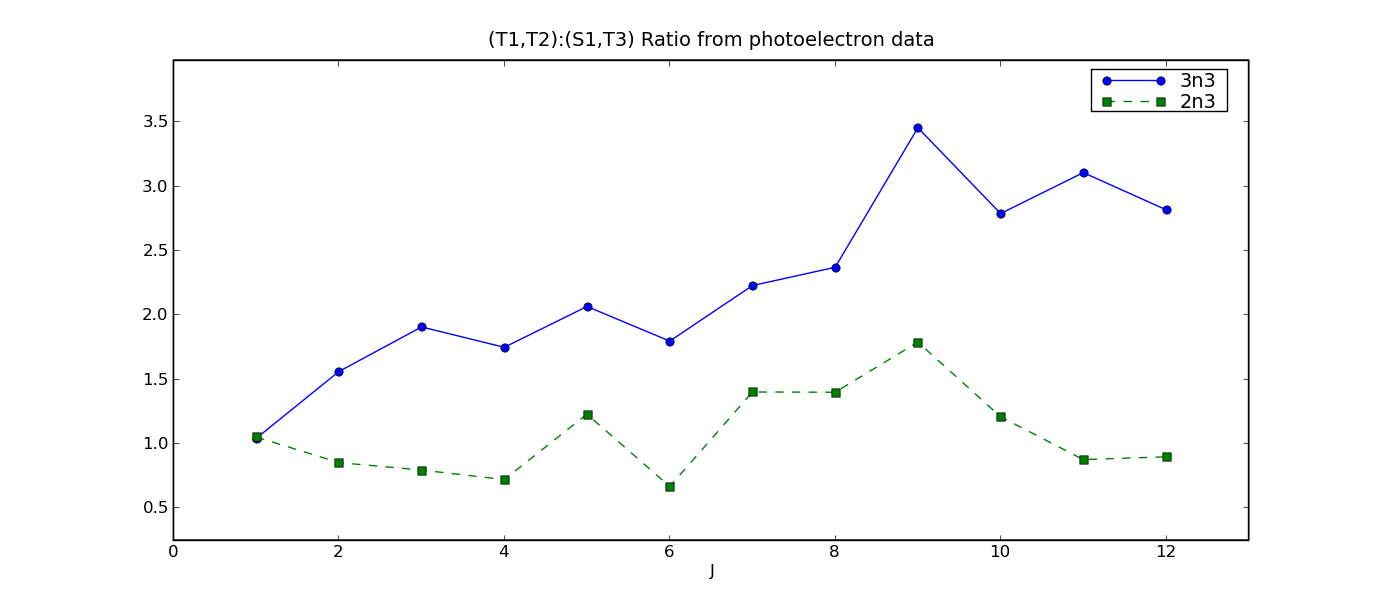
\includegraphics[width=7in]{mattijs-ratios.png}
  \caption{}
  \label{fig:mattijs-ratios}
\end{figure}

\POINT{Discuss J-dependent effects in spin-orbit coupling and rule out
  other mechanisms (L-uncoupling) capable of producing the same
  effect. Terms including $B(L \cdot J)$ are diagonal in spin,
  increase linearly with $J$, and is a Coriolis-type interaction.
  Check Bob's book, Herzberg, and B\&J.  (see p.55 of 11/2007--1/2008
  notebook)}



\section{Experiment}

\POINT{Experimental procedures.  Chamber optics measurements on p.13
  of 9/2006--1/2007 notebook.}  The experimental apparatus has been
described previously.  \TODO{Cite apparatus papers and theses.}
Briefly, 355nm light from a 20Hz pulsed Nd:YAG laser (Spectra-Physics)
is used to pump a dye laser (Lambda-Physik FL3002) operating with
Coumarin 440.  The dye laser output is frequency doubled in a BBO
crystal to produce up to 1 mJ of radiation in the vicinity of 220nm.
Using an intracavity etalon, the (incoherent) frequency resolution of
the doubled radiation is approximately 0.006\rcm.

Pure acetylene (Matheson) is expanded without purification from a
pulsed valve (Jordan) at 10Hz into a differentially pumped vacuum
chamber.  During operation, the pressure in the ``source'' chamber is
10$^{-5}$ torr.  At a distance of 2cm from the nozzle, the laser beam
crosses the free jet of acetylene perpendicular to its direction of
flow.  Laser induced fluorescence is collected in this region by an
$f/4$ quartz lens system and filtered (UG-5) before it enters a
UV-sensitive photomultiplier (Hamamatsu R375).  The time-resolved
output from the photomultiplier tube is averaged on a digital
oscilloscope (Model\#) and transferred to a computer.

At a distance of 5cm from the nozzle, the molecular beam passes
through a 3mm skimmer and enters the SEELEM detection chamber.  The
SEELEM detector is located 34cm from the laser excitation region.  The
active detection hardware consists of a gold surface, heated to 300C, oriented
at a normal angle to the beam, and an electron multiplier (Model\#).
The entrance aperature of the electron multiplier is positioned
immediately adjacent to the gold surface at a perpendicular angle,
facing the area of intersection with the molecular beam.  The electron
signal from the multiplier is sent to a preamplifier/discriminator,
and the resulting electron counts are recorded on a separate computer
using a PCI counting hardware from WHERE?  The LIF and SEELEM
detection systems are kept in sync by means of a stepping motor, which
is triggered triggered from the LIF computer to periodically hit the
space bar on the SEELEM computer.

\POINT{Relate survival probability and lifetime. Give $R$ value for
  our SEELEM detector.  Show plot of $C_{S_1}$ vs. lifetime/survival
  probability for eigenstates of acetylene.  (See p.97 of
  8/2007--10/2007 notebook.)}

\section{Results: new and revised assignments}

\TODO{Prepare a comparison to the Au:SEELEM data from our own lab, with
integrated intensities out to $J' = 7$.}

\TODO{Figure: integrated LIF + SEELEM intensities from our data.}



A more extensive and detailed Au:SEELEM/LIF spectrum has been recorded
in the vicinity of the $V^3_0K^1_0$ subband. This data set covers the
upper state energy levels $J'=1-8$, from 45273.3 to 45314.7 \rcm.

\POINT{Present overview of spectrum.  Compare with R\&A dataset.}

\TODO{Figure: spectrum overview.}

\TODO{Figure: SEELEM comparison with R\&A. (see p.56 in
  11/2007--1/2008 notebook)}

\POINT{Explain gated fluorescence measurements and present theory.}

\TODO{Figure: example of gated fluorescence spectrum.}

\POINT{Assignment of LIF and SEELEM features by ground state
  combination differences.}

\TODO{Figure: Show each line and its combination difference for LIF
  and SEELEM.  Explain what qualities must be preserved between the
  two energy regions.  See p.110,128,138 of 9/2006--1/2007 notebook.}

\POINT{Present the spectrum of $4^1 6^3$, the complimentary member of
  the $B^4$ polyad, and show that it has no appreciable SEELEM
  intensity + a short lifetime. (Scan on 2/2/07)}

\subsection{Assignments revised from Mishra \emph{et. al.}}

\POINT{Measurement of fluorescence lifetimes has led to many
  corrections to the assignments in Mishra \emph{et. al.}}

\subsubsection{Mis-assignments of triplet transitions}

As stated in [Ryan \& Bryan], the transitions assigned to the O(3,4,5)
of $T_3$ were later observed to have short lifetimes, therefore this
assignment cannot be correct.  The S(1) transition assigned in [MTF]
at 45310.397 \rcm has been re-assigned as R(4) after careful
comparison with ground state combination differences.  This
re-assignment slightly changes the rotational constant for the triplet
perturber inferred from the reduced term value plot.

The singlet pertuber line R$_e$(3) was mis-assigned as $T_3$ R(4).
This transition has a short fluorescence lifetime and a ground state
combination difference with a P$_e$(5) transition at 45289.69 \rcm.
(The $S_1$ Q(9) transition partially overlaps this P$_e$(5) line.)
This new assignment is reflected in the reduced term value plot.  Our
gated fluorescence method allows us to observe R$_e$(4), which is
partially overlapped with the blue end of the $S_1$ R(6) cluster.

\TODO{Adapt reduced term value plot, page 132 of 8/2007--10/2007
  notebook.}

\POINT{This kills all the $\Delta N=\pm 1$ triplet transitions, so the
  $K$ assignment of the triplet perturber is called into question.
  Discuss what this affects.}

\POINT{Combination differences killed to O and S branches, therefore
  we return to $N$-only assignments in the lack of other evidence.
  Lines assigned to triplet perturbers Q(1) $J'=2$ and Q(2) $J'=3$ are
  blended, according to Drabbels.  Lines assigned to Q(2) $J'=1$ and
  Q(3) $J'=2$ are mis-assigned, disagree with Drabbels assignments
  based on relative intensity at different beam temperatures.}

We still retain the assignment of the triplet perturber as the $F_2$
($N=J$) component, because an $F_1$ or $F_3$ component would not be
nearly degenerate with the singlet level over several consecutive $N$.
By a process of elimination, this leads to the conclusion that the
local triplet perturber must have $K_T=1$.  A triplet level with
$K_T=0$ would interact with only one parity of the \sing $K=1$ level,
and such a perturbation would be observed exclusively in \emph{either}
the Q or (P, R) branches.  The local $T_3$ perturbation is present in
all three branches, thus it must have $K_T\ne0$.  A triplet perturber
with $K_T=2$ would have no rotational level with $J=N=1$, however such
a level perturbs the $J=1$ levels of \sing in both parities.  We
have thus eliminated all possibilities but $K_T=1$.

\TODO{Re-create figure from page 133 of 8/2007--10/2007 notebook.}

\subsubsection{Mis-assignments of singlet transitions}

The lines at 45298.262 and 45291.818 \rcm, assigned to Q(1) transitions of
$S_1(2\nu_4' + 2\nu_6')-S_0(K^1_0)$, have also been re-assigned due to long
lifetimes.  The former line is re-assigned as part of the fractionated
\strans Q(4) cluster.  The energy of the latter line
agrees with previous observations of the \strans Q(8) transition.

\POINT{The singlet perturber has basically been definitively assigned
  as $3\nu_4'+\nu_6'$.  This accounts for the large rotational
  constant, because torsional motion raises the effective B value.
  What else does this mean for the analysis in [MTF]?}

The lines previously assigned to the \fftrans Q(1,2,3) all have long
lifetimes, which precludes their assignment to a pure bending polyad.
For the lines at 45298.262 and 45297.999 \rcm, we return to the
Drabbels assignment of the \strans Q(4) cluster.  On the basis of
lifetime and temperature dependence, we re-assign the line at
45296.332 to the \strans Q(5) cluster.  The line prevoiusly assigned
as \fftrans Q(4) does have a short lifetime, but cannot be assigned
conclusively in light of the current data.

The assignment of the $S_14\nu_6'-S_0(K_0^0)$ Q-branch is also called
into question by the current data.  The lines assigned to Q(1) and
Q(4) are overlapped with the \sing Q(8) and Q(9) clusters in the
current data, and so cannot be commented on.  One of the two remaining
lines, assigned to Q(2), has a long lifetime, and therefore cannot be
assigned as a singlet perturber.  The line at 45290.401 \rcm,
previously assigned to Q(3), has a short lifetime, but cannot be
assigned conclusively in light of the current data.




\begin{table}
  \caption{Revised assignments in the LIF spectrum of $V^3_0K^1_0$.}
  \label{table:lif-assignments}
  \centering
  \subfloat{
    \begin{tabular}[t]{l r l}
      \toprule
      Assignment & Energy & Intensity \\
      \midrule
      $R(0)$ 
      & 45302.716 \\
      &     2.881 \\
      &     3.186 \\[5pt]

      $R_e(0)$ 
      &     3.568 \\
      &     3.657 \\[12pt]     

      $R(1)$ 
      & 45304.440 \\
      &     4.651 \\
      &     4.750 \\
      &     4.973 \\
      &     5.085 \\
      &     5.246 \\
      &     5.333 \\[5pt]

      $R_e(1)$
      &     5.991 \\
      &     6.200 \\[12pt]


      $R(2)$ 
      & 45306.977 \\
      &     7.062 \\
      &     7.295 \\
      &     7.613 \\[12pt]
      
      $R_e(2)$
      &     8.360 \\
      \bottomrule
    \end{tabular}}
  \hspace{1cm}
  \subfloat{
    \begin{tabular}[t]{l r l}
      \toprule
      Assignment & Energy & Intensity \\
      \midrule
      $R(3)$ 
      & 45308.495 \\
      &     8.765 \\
      &     8.975 \\
      &     9.222 \\
      &     9.297 \\[5pt]

      $R_e(3)$
      &    10.866 \\[12pt]

      $R(4)$ 
      & 45310.335 \\
      &    10.397 \\
      &    10.594 \\[5pt]

      $R_e(4)$
      &    13.573 \\[12pt]

      $R(5)$ 
      & 45311.620 \\
      &    11.818 \\
      &    12.053 \\
      &    12.177 \\
      &    12.473 \\[12pt]

      $R(6)$ 
      & 45313.153 \\
      &    13.240 \\
      &    13.499 \\[12pt]

      $R(7)$ 
      & 45314.278 \\
      &    14.389 \\
      \bottomrule
    \end{tabular}
  }
\end{table}

\begin{table}
  \caption{Revised assignments in the Au:SEELEM spectrum of
    $V^3_0K^1_0$. Transition energy is given in units of cm$^{-1}$. 
    The intensity is given in electron counts per 100 laser shots.}
  \label{table:seelem-assignments}
  \centering
  \subfloat{
    \begin{tabular}[t]{l r r}
      \toprule
      Assignment & Energy & Intensity \\
      \midrule
R(0) & 45301.584 \\
     &     1.864 \\
     &     2.029 \\
     &     2.271 \\
     &     2.449 \\
     &     2.601 \\
     &     2.741 \\
     &     2.894 \\
     \cmidrule{2-2}
     &     3.212 \\
     &     3.301 \\
     &     3.644 \\[9pt]
    
R(1) & 45303.733 \\
     &     4.471 \\
     &     4.585 \\
     &     4.661 \\
     &     4.763 \\
     &     4.890 \\
     &     4.954 \\
     &     5.005 \\
     &     5.081 \\
     &     5.119 \\
     &     5.221 \\
     \cmidrule{2-2}         
     &     5.348 \\
     &     6.225 \\
     \bottomrule
   \end{tabular}}
 \subfloat{
   \begin{tabular}[t]{l r r}
     \toprule
     Assignment & Energy & Intensity \\
     \midrule
R(2) & 45306.474 \\
     &     6.964 \\
     &     7.062 \\
     \cmidrule{2-2}
     &     7.136 \\
     &     7.319 \\
     &     7.613 \\[9pt]

R(3) & 45308.495 \\
     &     8.569 \\
     &     8.765 \\
     \cmidrule{2-2}
     &     8.839 \\
     &     8.926 \\
     &     8.987 \\
     &     9.049 \\
     &     9.173 \\
     &     9.247 \\
     &     9.321 \\
     &     9.445 \\
     &     9.519 \\
     &     9.580 \\
     &     9.852 \\
    \bottomrule
  \end{tabular}}
\end{table}

\POINT{Table~\ref{table:lif-assignments} shows new LIF assignments in the R-branch of \sing}

\POINT{Table~\ref{table:seelem-assignments} shows new SEELEM assignments in the R-branch of \sing}

\section{Analysis: Relative LIF-SEELEM intensity distributions}

\POINT{Discuss the integrated intensity results/moments of distributions
  for the SEELEM and LIF data. Focus on the data, and reference
  elsewhere the derivations of intensity distributions.}

\POINT{Show the systematic skew of the spectral intensity
  distribution.  Compare predicted skewness for single and double
  doorway models?}

\POINT{Must show conclusively that the intensity distributions are the
  same for LIF and SEELEM, therefore a SEELEM intensity cross term
  cannot account for the skewness.  Avoid direct reference to SEELEM
  de-excitation mechanisms.  (If you must discuss them, see p.7 of
  8/2007--10/2007 notebook.)}

\POINT{Address the change in various parameters with mixing
  coefficient under a single or double doorway model. (See p.41 of
  11/2007--1/2008 notebook.)}

\begin{table}
  \centering
  \caption{}
  \label{table:seelem-intensity-ratios}
  \begin{tabular}[t]{l r r r l}
    \toprule
    Assignment & Window & Counts$_<$ & Counts$_>$ & Ratio \\
    \midrule
    R(0) & 1.0 & 263014 & 202732 & 1.30 \\
    R(1) & 1.0 & 433225	& 191193 & 2.27 \\
    R(2) & 0.7 &  96684 &  88121 & 1.10 \\
    R(3) & 1.0 & 114986 & 185850 & 0.62 \\
    R(4) & 0.7 &  27116 &  22422 & 1.21 \\
    R(5) & 0.5 &  30252 &  26668 & 1.13 \\
    R(6) & 0.5 &  12711 &  11619 & 1.09 \\
    R(7) & 0.4 &   5638 &   5105 & 1.10 \\
    \bottomrule
  \end{tabular}
\end{table}

Table~\ref{table:seelem-intensity-ratios} presents intensity ratios on
either side of the nominal bright state.

\POINT{Fractionation arguments - F-value should be the same on either
  side of the nominal bright state. States cannot change
  order. Support this argument with evidence from simulations. Can the
  variance of the F-value be derived from the assumption of direct
  coupling and the average matrix element?}

\begin{figure}
  \caption{}
  \label{fig:f-seelem}
  \centering
  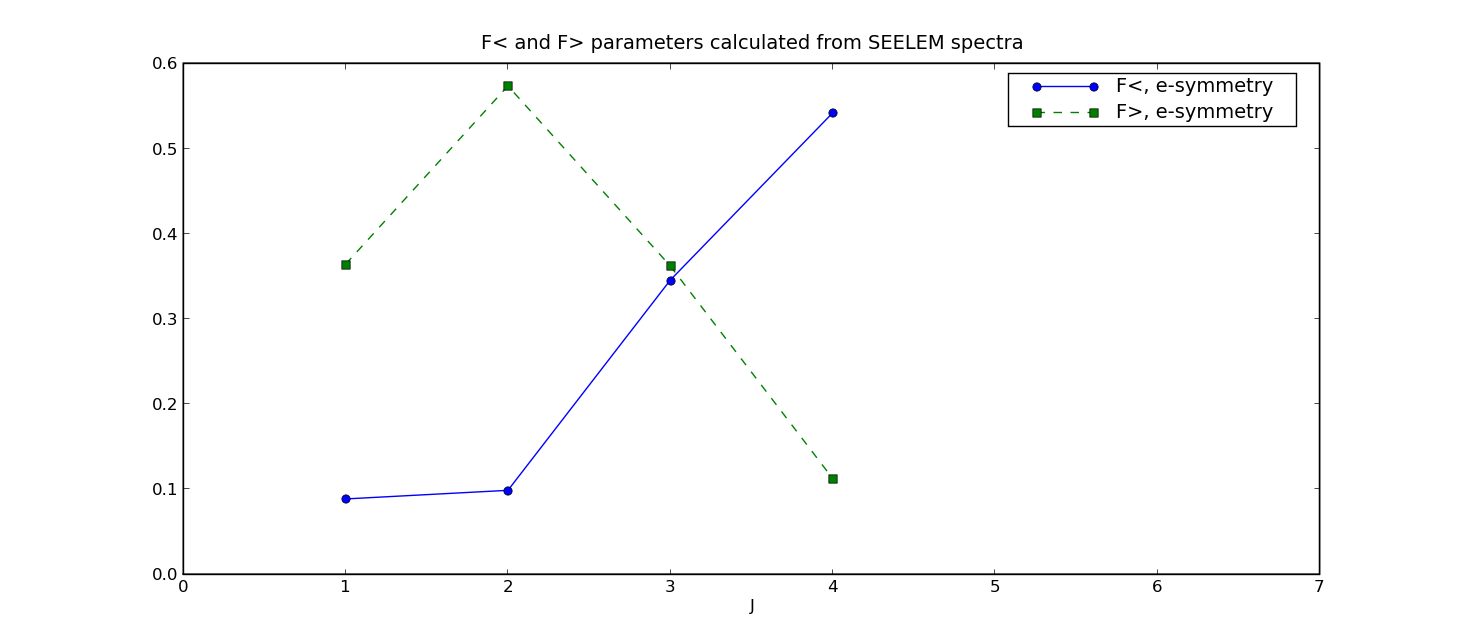
\includegraphics[width=7in]{f-seelem.png}
\end{figure}

Figure~\ref{fig:f-seelem} shows the fractionation on either side of
the nominal bright state.

\section{Analysis: Deconvolution and deperturbation}

\POINT{Present full deconvolution results.}

\POINT{Perform a continuous deconvolution for $J'=5-8$.}

\TODO{Figure: matrix elements and dE's from a LK deconvolution.}

\POINT{Use deconvolution results to place $S_1 \sim T_3$ interaction
  in the spectrum of weak coupling -- strong coupling. Is a ``nominal
  doorway state'' observed in the spectrum?  How close is its
  intensity to the mixing fraction $\alpha^2$?  What total amount of
  singlet character is borrowed by nominal $T_{1,2}$ states?}

\section{Analysis: Parsimonious trees}

\POINT{Examine the LIF and SEELEM spectra using parsimonious trees.
  Show that certain matrix elements keep popping up, and speculate on
  what this means.  The results will probably not be conclusive, but
  the previous sections should lend them some more weight.}

\section{Discussion: A local+distant ``double doorway'' model}

\POINT{What does the double doorway model mean for the rotational
  constant of the local perturber?  Could this account for the
  observed reversal of rotational constants for the two asymmetry ($e$
  and $f$) components?}

\POINT{Prepare and discuss a ``two slit'' figure for the double
  doorway model. (See p.43--45 of 11/2007--1/2008 notebook.)}

\section{Conclusions}

\begin{quote}
  Can there be anything left to say about this band?
\end{quote}

\begin{quote}
  We'll talk about where the distant doorway might be, and how it
  would appear in the spectrum.
\end{quote}

\end{document}